\section{Motion Planning Action Service(Catherine)}

%Motivation (why did you do it, who should care about it)
%Clearly state your contributions
%Technical details of what you did, with a focus on what's novel.
%Experimental results (if you did any experiments)
%Discussion (what is interesting about the results)

%This component is divided into two subsections:
%\begin{enumerate}%[label=\thesection.\arabic*]
%\item Trajectory Planner for robot arm trajectory planning, and
%\item Trajectory Executor for robot arm trajectory execution.
%\end{enumerate}

The motion planning action service can be separated into three components as shown in Fig.~\ref{fig:plan}.

\begin{figure}[ht!]%[H]
\centering
{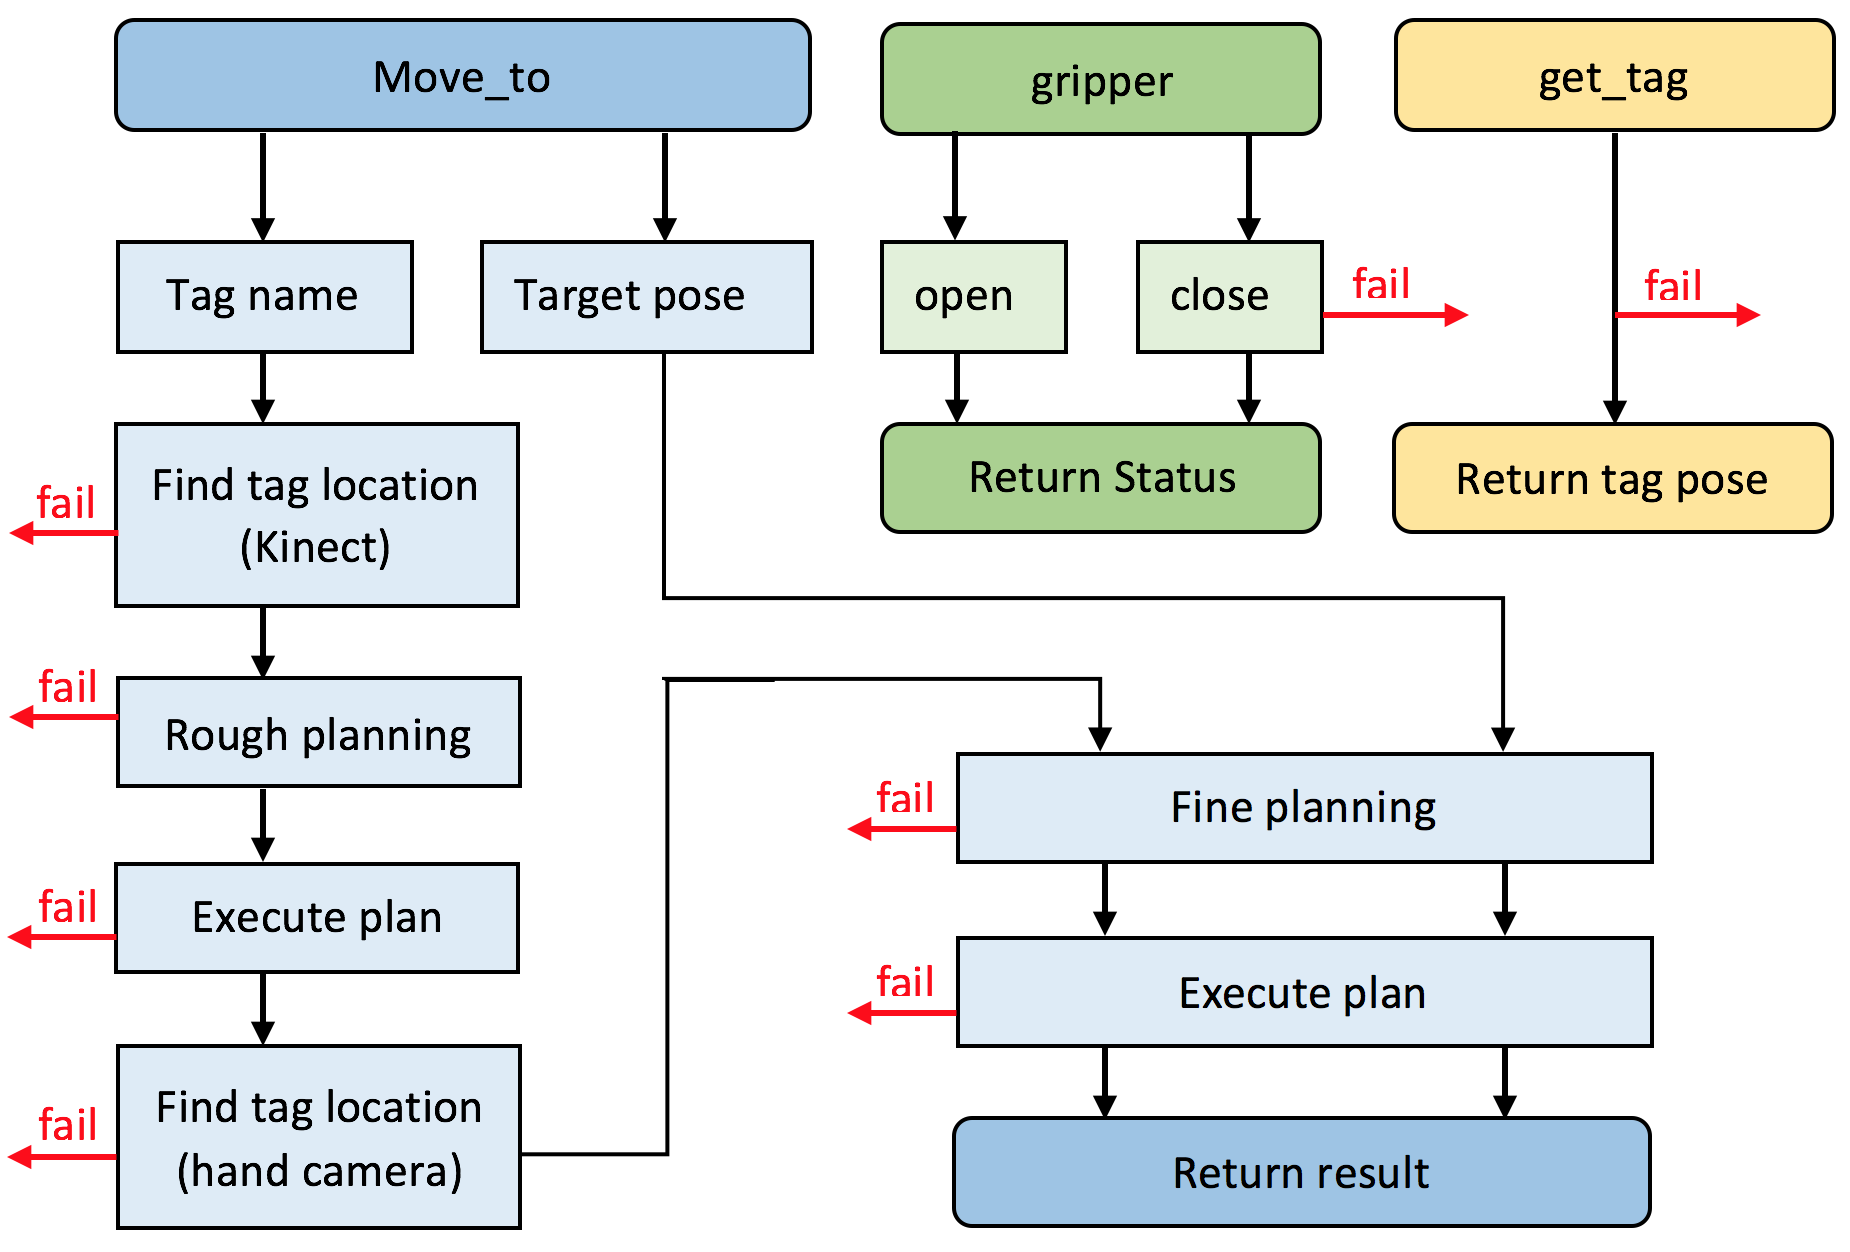
\includegraphics[width=0.95\columnwidth]{pics/motion_planning_flow.png}}
\caption{Motion Planning Action Service}
\label{fig:plan}
\end{figure}

The motion planning action service is an action service in ROS and based on the action types: move\_to, gripper or get\_tag, the service executes different actions and returns requested information.

\subsection{Trajectory Planner (move\_to component)}

During execution, the task planner requests the path planner to create trajectory plans for one or more robot arms. The planner aims to find a plan that (i) each arm starts at its initial configuration, and (ii) each arm ends with each robot end effector within a certain distance from the final desired workspace position. 

There are a variety of path planning algorithms developed in the community~\cite{DBLP:books/daglib/0016830} and some algorithms are adapted for finding robot arm trajectories. 
Researchers have proposed sampling-based approaches with probabilistic completeness such as the Rapidly-Exploring Random Tree (RRT) algorithm~\cite{VahrenkampBAKD09} to find trajectories for robot arms. Others have used Probabilistic RoadMaps (PRM) that work with high-dimensional spaces~\cite{KavrakiSLO96} but this algorithm requires pre-computation of the roadmap and no dynamic obstacles in the environment. In this work, we do not conduct pre-processing and the other arms can temporarily be obstacles in the environment. As a result, we are using an improved version of RRT, RRT-Connect~\cite{KuffnerL00} to find trajectories for the robot arms.


Our work leverages the existing open-source planning software for manipulation, MoveIt! \cite{moveit} with the Open Motion Planning Library (OMPL)~\cite{sucan2012the-open-motion-planning-library} to plan trajectories for the robot arms. 


\subsubsection{Objects to Avoid in Trajectory Planning}~\\
The major objects to avoid in path planning are the table and all the modules excluding the target module, as shown in Fig.~\ref{fig:realBaxter}. In this project, we have explored two different ways to model objects in the world. 

\paragraph{Octamap}\label{obstacle-octamap}
For our first attempt, we subscribe to the depth information of a Kinect facing the robot and create an octamap around the robot. An octamap is a 3-D occupany grid that builds an obstacle map around the source, in this case the Kinect, and updates over time with new information of the evolving environment. Figure~\ref{fig:octamap} shows an example of the octamap around Baxter.

Since the modules are modeled as obstacles in the octamap, to approach and grasp the module, we remove the target module from the octamap through inserting a module-like scene object into the workspace (Fig.~\ref{fig:octamap_object}). The octamap automatically subtracts any scene objects and by excluding the module object from collision check during trajectory planning, MoveIt! can find a path to the module.

\paragraph{Table Object}\label{obstacle-table}
Since the environment of the workspace is given, the other way to model obstacles in the environment is simply adding a table object right in front of Baxter, as shown in Fig.~\ref{fig:table_only}. 

We compared the performance of the two approaches for modeling obstacles. It turned out clustering of modules could be a problem when using an octamap and MoveIt! could not find a plan. On the other hand, when we simply model the environment with only a table in front, the resulting plan may sometimes touch the other modules. Looking at Fig.~\ref{fig:table}, notice that the table object is a pretty good representation of the obstacle information from the octamap. Since the modules are movable in the workspace, we determined that it will be better to get a plan most of time and we go on with approach b) to model obstacles. 

%\quad
%\quad
\begin{figure*}[h]
%\begin{figure}[ht!]%[H]
\centering
\subfloat[Real Scenario of Baxter with modules on a table]{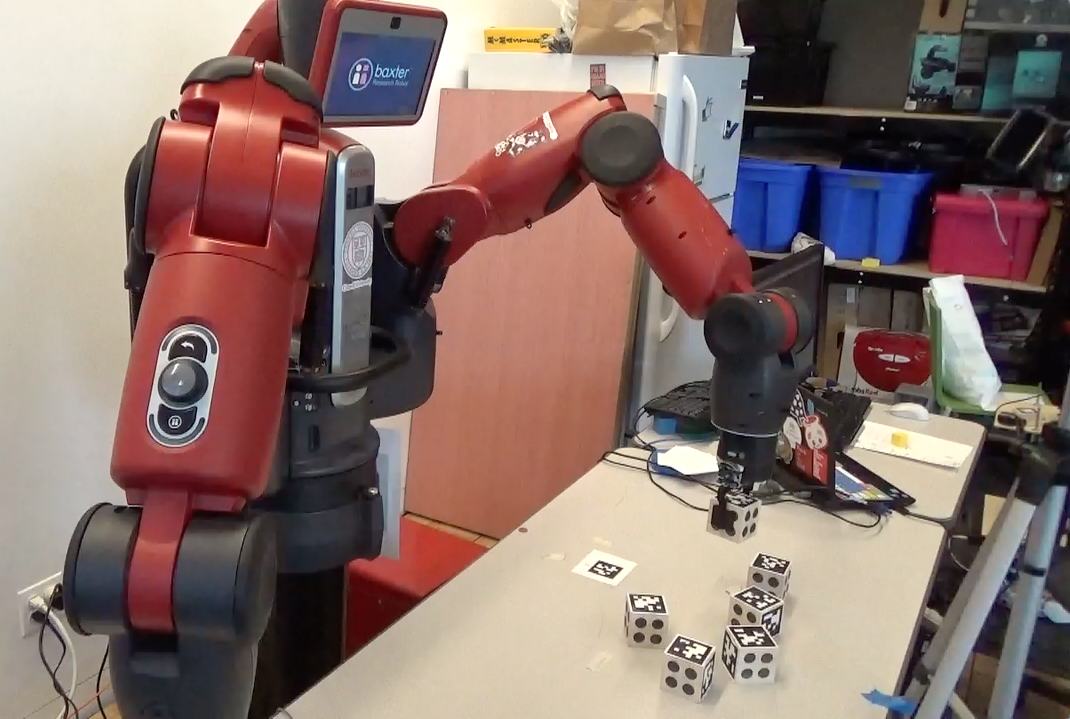
\includegraphics[width=0.35\columnwidth]{pics/baxter_real_table.png}\label{fig:realBaxter}}\hspace{0.1cm}
\subfloat[Octamap from depth data of Kinect in Rviz]{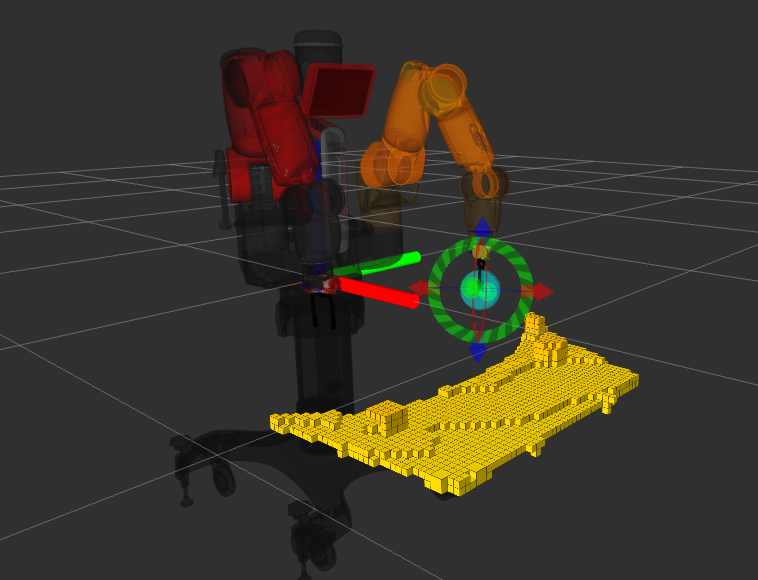
\includegraphics[width=0.35\columnwidth]{pics/baxter_with_octamap.png}\label{fig:octamap}}\hspace{0.1cm}
\subfloat[Octamap from depth data of Kinect with a module object inserted in Rviz]{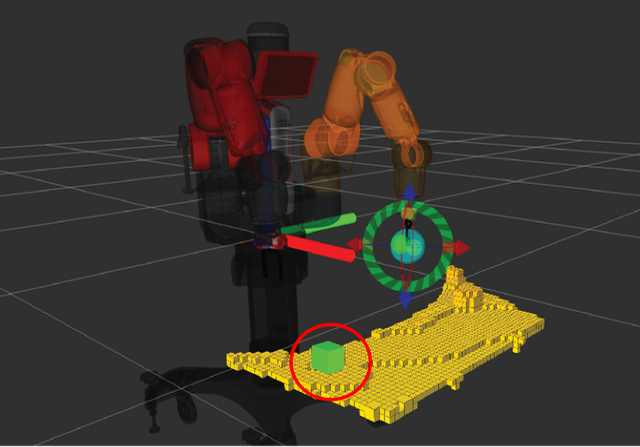
\includegraphics[width=0.35\columnwidth]{pics/baxter_octamap_with_object.png}\label{fig:octamap_object}}\hspace{0.1cm}
\subfloat[Table object inserted in Rviz as obstacle]{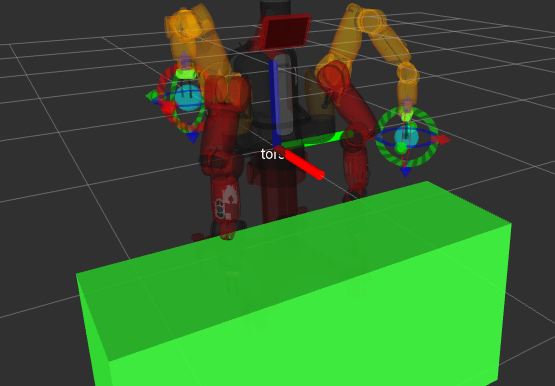
\includegraphics[width=0.35\columnwidth]{pics/baxter_with_table_only.png}\label{fig:table_only}}\hspace{0.1cm}
\subfloat[Octamap from depth data of Kinect with a table object inserted in Rviz]{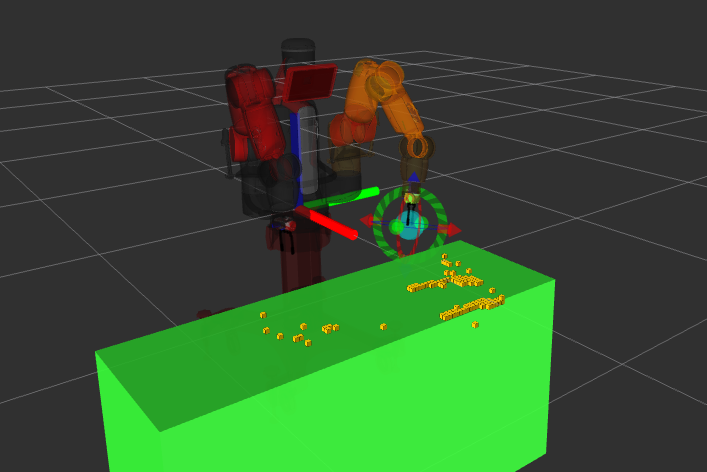
\includegraphics[width=0.35\columnwidth]{pics/baxter_with_table.png}\label{fig:table}}
\\
\caption{Modeling obstacles in trajectory planning}
\end{figure*}



\subsubsection {Transformation of Tag Pose to Gripper's Goal Pose}~\\
To plan an arm trajectory, the algorithm also requires the goal pose of the gripper to plan accordingly.  The goal pose can be separated into two components: the xyz-position of the pose ($p_{\mathrm{effector}}$) and the orientation of the pose ($q_{\mathrm{effector}}$) in the form of a quaternion.

The gripper goal pose comes from the target module pose, which consists of the position ($p_{\mathrm{tag}}$) and orientation of the module ($q_{\mathrm{tag}}$). For the goal position ($p_{\mathrm{effector}}$), it is either exactly the same as the tag position ($p_{\mathrm{tag}}$) or with a small offset ($p_{\mathrm{offset}}$) from the tag position. The goal position can be represented with the following equation:

%\begin{bmatrix}
%    \mathrm{offset}_{x} \\
%    \mathrm{offest}_{y} \\
%    \mathrm{offset}_{z}
%\end{bmatrix}
%+
%\begin{bmatrix}
%    \mathrm{tagPosition}_{x} \\
%    \mathrm{tagPosition}_{y} \\
%    \mathrm{tagPosition}_{z} \\
%\end{bmatrix}
\begin{equation}
p_{\mathrm{effector}}= p_{\mathrm{offset}}+p_{\mathrm{tag}}
\end{equation}

In this project, all the modules have z-axis pointing upwards. However, to grasp a module, the gripper should point downwards, i.e., z-axis of the gripper points downwards. To obtain the goal orientation ($q_{\mathrm{effector}}$), our system rotates the tag orientation about x-axis by $\pi$ radians, as shown in the following equation: 

\begin{equation}
q_{\mathrm{effector}}= q_{\mathrm{tag}}\: q_{\mathrm{zFlip}}\mathrm{,\ where\ } q_{\mathrm{zFlip}} =  (0, \mathbf{i})
\end{equation}


\subsubsection {Two-step Trajectory Planning}~\\
Through testing our approach, our group have noticed that the camera information from a Kinect sensor facing the 
\begin{wrapfigure}{r}{0.45\columnwidth}
\begin{center}
\vspace{-8pt}
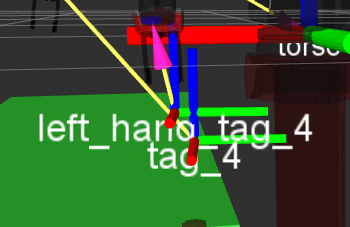
\includegraphics[width=0.45\columnwidth]{pics/kinect_tag_pose3_croped.png}
\caption{Differences in pose when using different sensor information.}
\label{fig:offTagPose}
\vspace{-12pt}
\end{center}
\end{wrapfigure}
robot does not give an accurate position of the modules using AprilTags recognition,  
as the distance from Kinect to the module increases. 
The position of the modules from Kinect is off by about 5cm and it is not good enough for the arm and gripper to arrive at the module location and grasp the module. Fig.~\ref{fig:offTagPose} shows the differences of tag pose when using the Kinect sensor (tag\_4) and the left hand camera (left\_hand\_tag\_4).

With this observation, in this work, we propose a two-step trajectory planning, which consists of a `rough' planning step and a `fine' planning step, and both steps leverage RRT to conduct the planning. 

From an arbitrary location, our system first conducts a `rough' planning to have the gripper arrive at a pose that is roughly above the module using the tag information from the Kinect sensor, with the gripper pointing downwards at the module.

Once the robot arms moves to the 'rough' location, now the robot  uses the camera on its hand to obtain a better location estimate of the module. With a more accurate location, the system then conduct a `fine' planning to the grasp location of the module. 

\subsubsection{Execute Trajectory}~\\
Once a trajectory is found through `rough' planning or `fine' planning, the action service executes the trajectory and returns the result.


\subsection{Open/Close Gripper (gripper component)}
When receiving a request to open and close gripper, the component executes the command and returns the result.

\subsection{Retrieve Module Pose (get\_tag component)}
Besides responding to different action requests, the action service can also get the pose of a module and return the pose to the client. With the pose, the client can transform the pose according to his or her needs and request trajectory planning with a given pose, as shown in Fig.~\ref{fig:plan} with command move\_to and a target pose.


\subsection{Failures}
Since the trajectory planning algorithm RRT is probabilistic complete, it may not find a path given a finite time horizon. It is useful to provide feedback to the client about the status of the request or that the planning failed. In our system, it returns not only the planning result but also the current process in execution to the client so that the client is always informed.

Besides the trajectory planner may not return or execute a plan, the gripping motion and the retrieveal of module pose can also fail. All these failure information are returned to the client, as shown with the red failed arrows in Fig.~\ref{fig:plan}.

\subsection{Results}
Compared to our plan in the proposal, we have successfully conducted trajectory planning for one arm and two arms simultaneously. The action service is also able to detect and report failure. In the future, we would like to extend our system to plan for four arms together. 

We have tried creating our version of RRT but modeling of the environment and checking collision between joints posed challenges. Since MoveIt! gives reliable results, our action service is using the software as the core planning interface.

We did not detail our plan to obtain target pose in the proposal but in the final result the action service is able to transform pose and return pose information. The action service can also respond to requests of opening and closing gripper.


%other attempts
%\begin{itemize}
%\item also tried broadcasting the goal location of the robot to tf and then fetch it, but then there is a lot of overhead and it will be easier doing transformation leveraging the tf.transformation module.
%\item also played with the inverse kinematic library (pyKDL) before but when switch it moveit, all the inverse kinematics are handled by Moveit.
%\item originally tried to generate waypoints of trajactory. To populate points on the RRT tree, but collision detection is using FCL but moveit set up the environment/scene so using moveit now.
%\item create object and then removing to from collision matrix. in this case, the robot can contact the object and the octamap is cleared at the point. The downside was the filtering wasn't good around the grippers. Also adding a table gives a close approximation. 
%\end{itemize}







